\documentclass{article}
\usepackage{graphicx} % Required for inserting images
\usepackage{float}
\usepackage[T1]{fontenc}
\usepackage{amsmath}
\usepackage[margin=1in]{geometry}
\usepackage{booktabs}
\usepackage{tabularx}
\usepackage[hidelinks]{hyperref}

\title{Raising the short band to +4 vol points on the short-only book}
\author{Experiment report \textperiodcentered{} L/S Gamma Desk, QUANTT}
\date{2026-10-16}

\begin{document}

\maketitle

\textbf{Question:} On the short-only book, does raising the short band from +2 to +4 vol points raise net P\&L at 1x and 2x spreads, in both halves, because each trade's edge rises more than the trade count falls?

\textbf{Method:}

\begin{itemize}

\item \textbf{Pre-registration:} the hypothesis card was committed before any run (commit 6b9adb9).

\item \textbf{Data:} the live paper rules (\texttt{configs/\allowbreak{}paper.\allowbreak{}toml}) are replayed on R2 replay snapshots v1 (config\_hash b040760187f0) over the development window 2014-06-02 to 2024-12-31. The hold-out (2025-01-01 to 2026-07-10) was not used.

\item \textbf{Book:} short-only (\texttt{[signal] long\_\allowbreak{}band = -\allowbreak{}inf}). That means a short put near 30 DTE, 1 contract, one position at a time, with the signal and hedge at 10:15 ET. A short opens when VRP (ATM IV minus the GARCH RV forecast) is above \texttt{short\_\allowbreak{}band}. It closes after 3 straight days at or below the band (flat exit), at 7 DTE, on the stop (1x credit) or at the 50\% profit-take.

\item \textbf{Variants:}

\begin{itemize}

\item \texttt{band4} (primary): \texttt{short\_\allowbreak{}band = 0.\allowbreak{}04}.

\item \texttt{band3} (sensitivity, reported only): \texttt{short\_\allowbreak{}band = 0.\allowbreak{}03}.

\item Reference \texttt{short\_\allowbreak{}only} (\texttt{short\_\allowbreak{}band = 0.\allowbreak{}02}): the registered runs of \texttt{2026-\allowbreak{}10-\allowbreak{}16-\allowbreak{}short-\allowbreak{}only/\allowbreak{}short\_\allowbreak{}only}, reused and not rerun. Their saved config matches the current config with \texttt{long\_\allowbreak{}band = -\allowbreak{}inf}.

\end{itemize}

\item \textbf{Runs:} each variant ran once at 1x and 2x spreads. Costs are \$0.65 per contract and \$0.005 per share, with a \$1 minimum per order. Baseline trial 1 (live rules, with longs) is shown in the charts for context only.

\end{itemize}

This report was written by Claude at the PM's request.

\section{Result vs the pass bar}

\texttt{band4} against \texttt{short\_\allowbreak{}only} at the same spread multiple. Every check had to hold at 1x and 2x. P\&L is net USD on daily equity for 1 contract. ES is the mean of the worst 5\% of daily P\&L.

\begin{center}\small
\begin{tabularx}{\linewidth}{>{\raggedright\arraybackslash}X l l l l >{\raggedright\arraybackslash}X}
\toprule
\textbf{Check} & \textbf{1x value} & \textbf{1x bar} & \textbf{2x value} & \textbf{2x bar} & \textbf{Result} \\
\midrule
Net P\&L, full window & \ensuremath{-}950 & > \ensuremath{-}774 & \ensuremath{-}1,525 & > \ensuremath{-}2,351 & fail 1x, pass 2x \\
Net P\&L, 2014-06 to 2019-12 & \ensuremath{-}237 & > \ensuremath{-}875 & \ensuremath{-}355 & > \ensuremath{-}1,261 & pass \\
Net P\&L, 2020-01 to 2024-12 & \ensuremath{-}713 & > +101 & \ensuremath{-}1,171 & > \ensuremath{-}1,090 & fail \\
abs ES 5\% \ensuremath{\leq} 1.10 \ensuremath{\times} reference & 61.7 & \ensuremath{\leq} 94.1 & 64.1 & \ensuremath{\leq} 101.7 & pass \\
Event floor: round trips (1x) & 53 & \ensuremath{\geq} 30 &  &  & met \\
\bottomrule
\end{tabularx}
\end{center}

\textbf{Verdict: failed.} Over the full window at 1x, the +4 band loses \$176 more than the reference. It also does worse in 2020-2024 at both spreads. It does better at 2x (+\$826) and in 2014-2019, mostly because it trades less. Every variant still loses money.

\subsection{Full-window numbers (not part of the bar)}

\begin{center}\small
\begin{tabularx}{\linewidth}{>{\raggedright\arraybackslash}X >{\raggedright\arraybackslash}X l l >{\raggedright\arraybackslash}X l l}
\toprule
\textbf{} & \textbf{short\_only 1x} & \textbf{band3 1x} & \textbf{band4 1x} & \textbf{short\_only 2x} & \textbf{band3 2x} & \textbf{band4 2x} \\
\midrule
Net P\&L & \ensuremath{-}774 & \ensuremath{-}546 & \ensuremath{-}950 & \ensuremath{-}2,351 & \ensuremath{-}1,658 & \ensuremath{-}1,525 \\
Round-trip P\&L before commissions & +318 & +1,252 & \ensuremath{-}66 & \ensuremath{-}1,240 & +156 & \ensuremath{-}630 \\
Net P\&L per round trip & \ensuremath{-}5.6 & +7.8 & \ensuremath{-}9.6 & \ensuremath{-}21.2 & \ensuremath{-}6.3 & \ensuremath{-}20.2 \\
Sharpe on \$250k & \ensuremath{-}0.15 & \ensuremath{-}0.11 & \ensuremath{-}0.24 & \ensuremath{-}0.42 & \ensuremath{-}0.33 & \ensuremath{-}0.38 \\
Max drawdown & 2,220 & 1,831 & 1,376 & 3,222 & 2,315 & 1,918 \\
ES 5\% (daily) & \ensuremath{-}85.5 & \ensuremath{-}73.1 & \ensuremath{-}61.7 & \ensuremath{-}92.4 & \ensuremath{-}77.9 & \ensuremath{-}64.1 \\
Round trips & 100 & 78 & 53 & 100 & 78 & 53 \\
Commissions (options /\allowbreak{} hedges) & 200 /\allowbreak{} 770 & 156 /\allowbreak{} 559 & 106 /\allowbreak{} 385 & 200 /\allowbreak{} 770 & 156 /\allowbreak{} 559 & 106 /\allowbreak{} 385 \\
\bottomrule
\end{tabularx}
\end{center}

The live-rules baseline (with longs) lost \$2,060 at 1x and \$4,122 at 2x.

\section{Charts}

\begin{figure}[H]\centering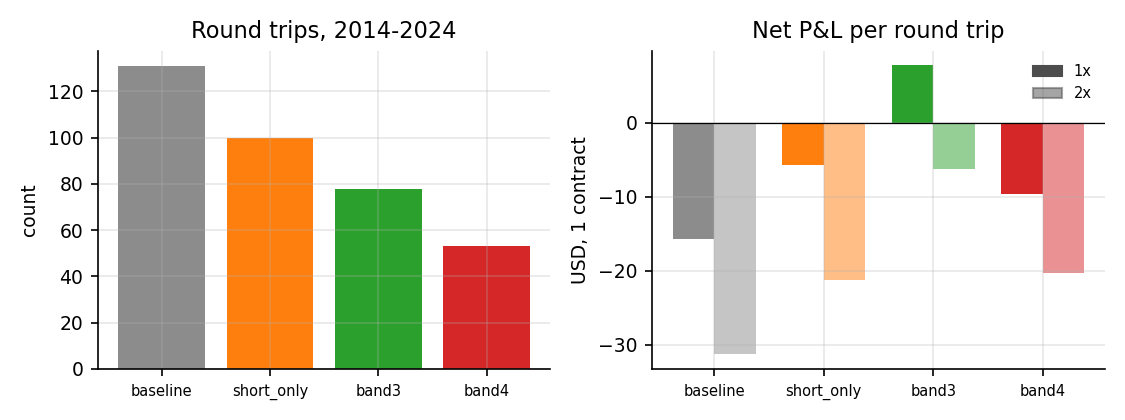
\includegraphics[width=0.92\linewidth]{figures/edge.png}\caption{Round trips and net P\&L per round trip (2x lighter)}\end{figure}

This chart shows the trade-off the hypothesis is about. Round trips fall from 100 to 78 at +3 and 53 at +4. At +4 the net edge per trade did not rise. It fell from \ensuremath{-}\$5.6 to \ensuremath{-}\$9.6 at 1x and was about the same at 2x (\ensuremath{-}\$20.2 against \ensuremath{-}\$21.2). The +3 band is the only book with a positive edge per trade at 1x (+\$7.8), but it is not the primary.

\begin{figure}[H]\centering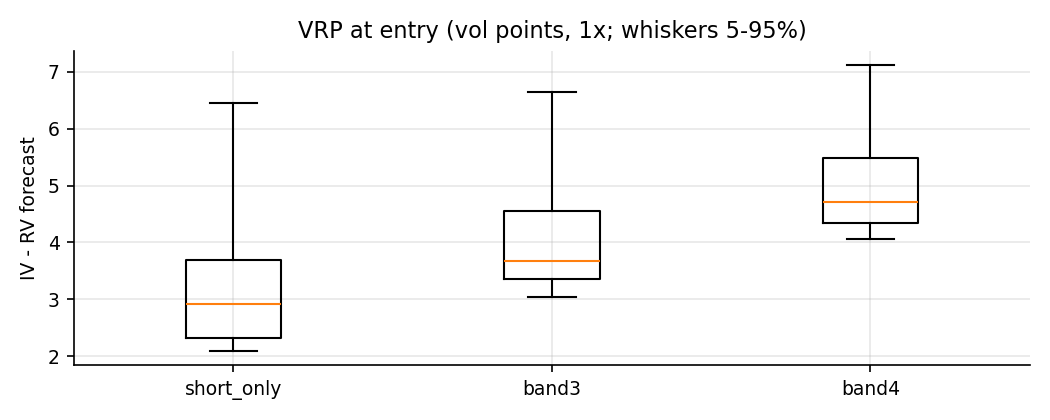
\includegraphics[width=0.92\linewidth]{figures/vrp_entry.png}\caption{VRP at entry, 1x (box: quartiles; whiskers: 5th-95th percentile)}\end{figure}

The band does select richer entries: the median VRP at entry rises from 2.9 to 3.7 and 4.7 vol points. So the entry filter works as intended. The problem is what happens after entry (see Analysis).

\begin{figure}[H]\centering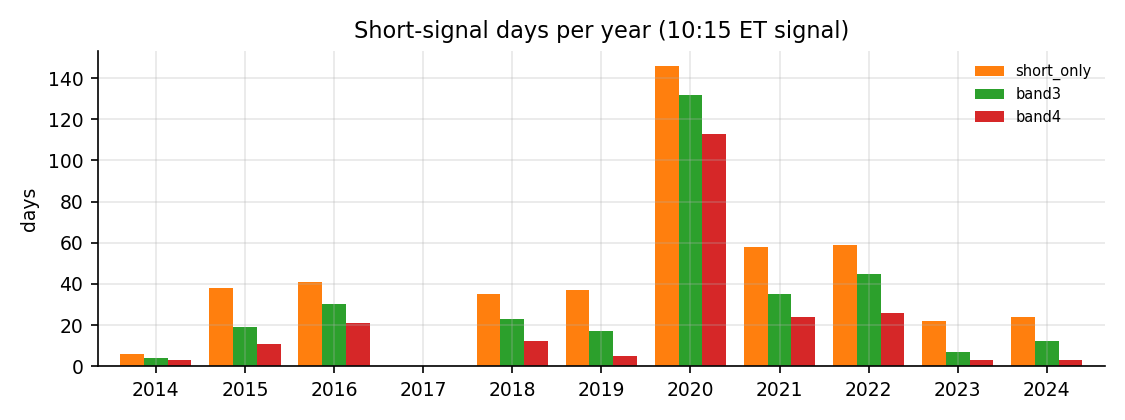
\includegraphics[width=0.92\linewidth]{figures/short_days.png}\caption{Short-signal days per year at the 10:15 ET signal}\end{figure}

Short-signal days fall from 466 to 324 at +3 and 221 at +4. A wider band thins the calm years most. At +4, 2019 has 5 short days and 2023 and 2024 have 3 each, while 2020 keeps 113 of its 146. No band has a short day in 2017. The +4 book holds a position on 350 of 2,576 trading days, against 716 for the reference.

\begin{figure}[H]\centering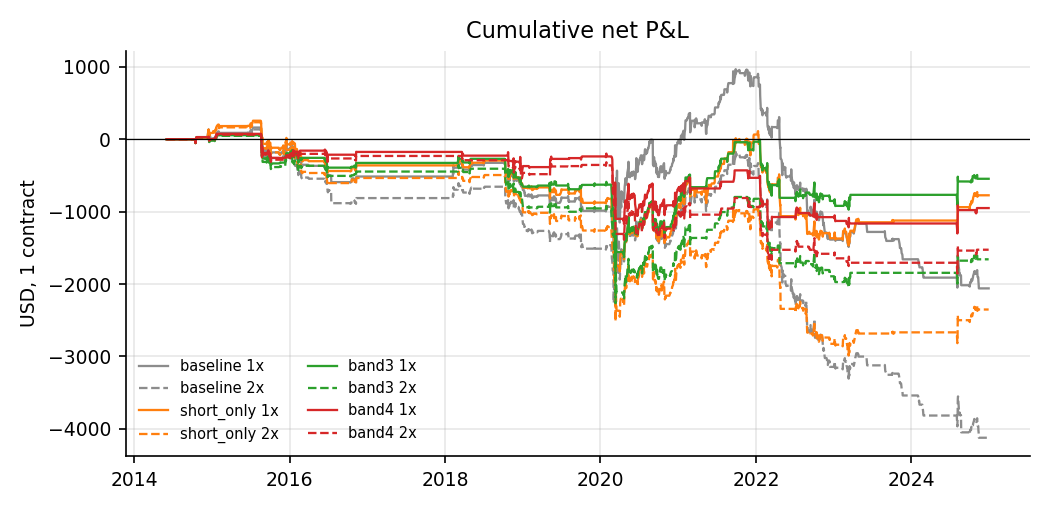
\includegraphics[width=0.92\linewidth]{figures/cum_pnl.png}\caption{Cumulative net P\&L, 1x solid and 2x dashed; baseline (live rules) grey}\end{figure}

Through 2019 \texttt{band4} loses less than the reference, because it sits out most of the calm years: \ensuremath{-}\$237 against \ensuremath{-}\$875 at 1x. In 2020-2021 it falls behind by about \$1,240 at 1x, then loses \$890 less in 2022. It ends \$176 behind at 1x. At 2x it stays ahead of the reference at every year-end from 2016 on. \texttt{band4} also has the smallest maximum drawdown at both spreads (\$1,376 at 1x against \$2,220), mostly because it holds a position on about half as many days. The drawdown and commission charts are in the experiment's \texttt{figures/\allowbreak{}} folder.

\begin{figure}[H]\centering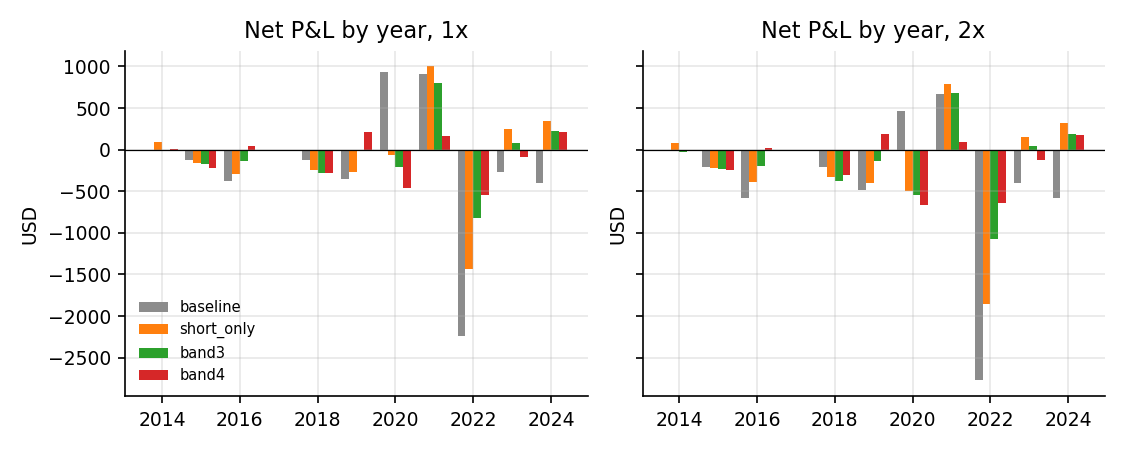
\includegraphics[width=0.92\linewidth]{figures/yearly.png}\caption{Net P\&L by year}\end{figure}

At 1x, \texttt{band4} beats the reference in 2016 (+\$46 against \ensuremath{-}\$291), 2019 (+\$218 against \ensuremath{-}\$270) and 2022 (\ensuremath{-}\$543 against \ensuremath{-}\$1,433). It falls behind in 2020 (\ensuremath{-}\$461 against \ensuremath{-}\$60), 2021 (+\$165 against +\$1,000), 2023 (\ensuremath{-}\$87 against +\$244) and 2024 (+\$213 against +\$349). Most of the 2020-2024 failure is in 2020-2021: \ensuremath{-}\$1,236 together, of which \$890 comes back in 2022.

\begin{figure}[H]\centering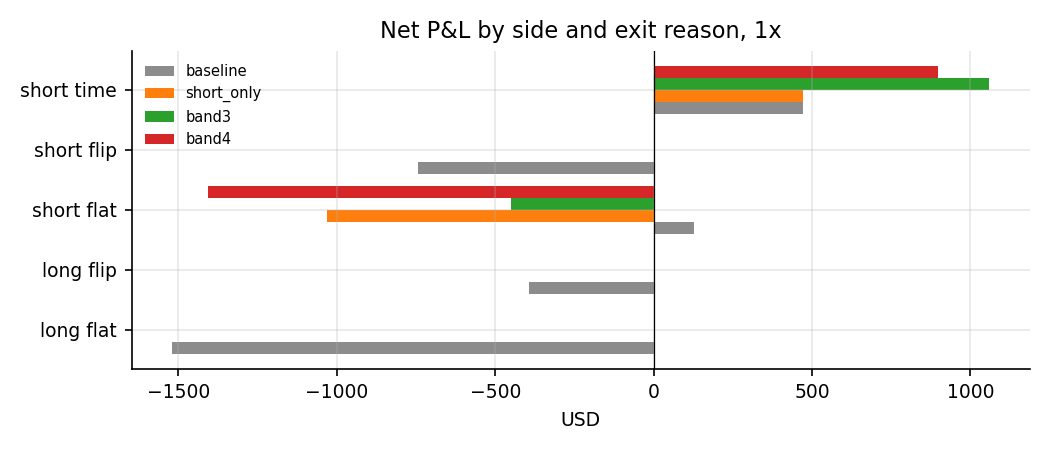
\includegraphics[width=0.92\linewidth]{figures/by_reason.png}\caption{Net P\&L by side and exit reason, 1x}\end{figure}

In every short-only book, only flat and time exits fire. At +4, the 48 flat exits lose \$1,406 net, or \ensuremath{-}\$29.3 each (\ensuremath{-}\$11.9 in the reference). The 5 time exits make +\$898, or +\$180 each (+\$36 in the reference). Time exits earn more per trade as the band widens, but fewer trades reach them.

\section{Analysis}

\subsection{Bridge from the reference to band4}

Equity P\&L splits into three parts:

\begin{enumerate}

\item \textbf{Round-trip P\&L before commissions.} This is already net of the spreads paid inside each trip.

\item \textbf{Commissions attributed to round trips.}

\item \textbf{The unattributed unwind residual,} which is equity P\&L minus round-trip net P\&L. Here it is exactly the order that flattens the hedge after each close without a same-time re-entry. That order costs a \$1 commission plus the gap between the fill-window price and the decision spot, times the shares.

\end{enumerate}

\begin{center}\small
\begin{tabularx}{\linewidth}{>{\raggedright\arraybackslash}X l l l l}
\toprule
\textbf{Change vs short\_only} & \textbf{band4 1x} & \textbf{band4 2x} & \textbf{band3 1x} & \textbf{band3 2x} \\
\midrule
Round-trip P\&L before commissions & \ensuremath{-}384 & +610 & +934 & +1,395 \\
Commissions in round trips (saved) & +438 & +438 & +237 & +237 \\
Unwind residual & \ensuremath{-}230 & \ensuremath{-}222 & \ensuremath{-}943 & \ensuremath{-}939 \\
\textbf{Net P\&L change} & \textbf{\ensuremath{-}176} & \textbf{+826} & \textbf{+228} & \textbf{+693} \\
\bottomrule
\end{tabularx}
\end{center}

At 1x the +4 band saves \$438 in commissions but loses \$384 of round-trip P\&L and \$230 in unwinds. At 2x the spreads paid inside each round trip double, so trading half as often saves more. Going from 1x to 2x costs \texttt{band4} \$575 of net P\&L, against \$1,578 for the reference. That is why 2x passes and 1x does not. The 2x gain comes from avoiding costs, not from more edge per trade.

\subsection{Why the edge per trade did not rise}

The band does two jobs. It is the entry threshold, and it is also the flat-exit threshold: a short closes after 3 straight days with VRP at or below the band. Raising the band to +4 selects richer entries. But it also closes them as soon as VRP drifts back into the +2 to +4 range, where the reference would keep holding.

The 17 \texttt{band4} trades that opened on the same day as a reference trade show this directly. All of them are reference entries with VRP above +4.

\begin{itemize}

\item \textbf{Exits.} In \texttt{band4}, all 17 closed on the flat exit after 8.4 days on average. In the reference, the same entries were held 14.1 days, and 4 of them reached the time exit. Only 5 of the 17 closed at the same time in both books.

\item \textbf{P\&L.} The same 17 entries made \ensuremath{-}\$858 before commissions in \texttt{band4}, against +\$194 in the reference (\ensuremath{-}\$988 against +\$8 net at 1x).

\item \textbf{Timing.} 7 of the 17 opened in 2020.

\end{itemize}

So the hypothesis's mechanism was half right. In the reference, by VRP at entry (1x):

\begin{center}\small
\begin{tabularx}{\linewidth}{l l >{\raggedright\arraybackslash}X}
\toprule
\textbf{VRP at entry} & \textbf{Trades} & \textbf{Net per trade} \\
\midrule
Above +4 & 22 & +\$44 (+\$963 in total) \\
+3 to +4 & 27 & \ensuremath{-}\$40 \\
+2 to +3 & 51 & \ensuremath{-}\$8.5 \\
\bottomrule
\end{tabularx}
\end{center}

The selection effect rests on very few trades, though. \$954 of the +\$963 came from 5 trades that \texttt{band4} did not open on the same day. And a band that also governs exits throws much of the effect away. This part is mechanical, not noise: it follows from the flat exit counting days against the same band.

\subsection{The unwind residual is noise, and it moves band3 most}

\begin{itemize}

\item \textbf{\texttt{band4}.} 49 unwind orders averaging 46 shares, with a price gap of \ensuremath{-}\$393. The five worst total \ensuremath{-}\$728, more than the whole \ensuremath{-}\$393.

\item \textbf{Reference.} 90 unwind orders averaging 44 shares, with a price gap of \ensuremath{-}\$122.

\item \textbf{\texttt{band3}.} A price gap of \ensuremath{-}\$1,083, of which \ensuremath{-}\$780 is in 2020 and 2022; the five worst total \ensuremath{-}\$991.

\end{itemize}

Without the residual, \texttt{band3}'s round trips netted +\$609 at 1x, against \ensuremath{-}\$562 for the reference. That is the only sign of real edge per trade in this test. But \texttt{band3} is a sensitivity variant and is not judged, and a handful of fills decides it.

\section{Verdict}

\textbf{Failed} on the pre-registered bar: the 1x full window fails, and so does the 2020-2024 half at both spreads. Keep the live +2 short band on the short-only book.

A possible follow-up would separate the entry band from the flat-exit band, for example entering above +4 but counting flat days only below +2. That tests the selection effect without the earlier exits. It needs its own card and a research-only engine flag, and it is in-sample. The reference trades above +4 suggest it, but there are only 22 of them, and 5 earn most of the profit.

\section{Caveats}

\begin{itemize}

\item \textbf{In-sample:} the idea comes from the 2026-10-16 desk discussion of the baseline on this same window. The VRP-bucket breakdown above is also in-sample.

\item \textbf{One contract:} the \$1 minimum per order is large relative to size. It favours books that trade less, which is part of the 2x result.

\item \textbf{Spread model:} fitted on about two weeks of calm 2026 live quotes; the 2x run is the stress test.

\item \textbf{Data gaps:} R2 has no month-end weekdays, so 89 scheduled times (3.3\%) are skipped in every variant.

\item \textbf{Few events:} \texttt{band4} made 53 round trips (20 in 2014-2019, 33 in 2020-2024) and had only 5 time exits. Each yearly difference rests on a handful of trades.

\item \textbf{ES is on daily equity, including flat days:} a book that is out of the market more often has a smaller ES almost by construction. The \texttt{band4} ES in 2014-2019 is \ensuremath{-}\$1.3.

\item \textbf{Path dependence:} with one position slot, a different band shifts every later entry, so only 17 of the 53 trades can be compared directly.

\end{itemize}

\section{Trials}

4 trials for this experiment: 2 variants at 1x and 2x, from one run of \texttt{experiment.\allowbreak{}py} at commit 6b9adb9, with no \texttt{-\allowbreak{}dirty} tag. The \texttt{short\_\allowbreak{}only} reference was reused from \texttt{2026-\allowbreak{}10-\allowbreak{}16-\allowbreak{}short-\allowbreak{}only} (2 trials, not rerun). The baseline has 2 trials. The pass bar was not changed.

\end{document}
